\documentclass[conference]{IEEEtran}
\IEEEoverridecommandlockouts
% The preceding line is only needed to identify funding in the first footnote. If that is unneeded, please comment it out.
\usepackage{cite}
\usepackage{amsmath,amssymb,amsfonts}
\usepackage{algorithmic}
\usepackage{graphicx}
\usepackage{textcomp}
\usepackage{xcolor}
\usepackage{ctex}
\usepackage{fancyhdr}
\begin{document}

\title{Image Colorization: A Survey\\
% {\footnotesize \textsuperscript{*}Note: Sub-titles are not captured in Xplore and
% should not be used}
}
\author{\IEEEauthorblockN{servuskk} 
\IEEEauthorblockA{allesgutewh@gmail.com}
}

\maketitle
\thispagestyle{fancy}
\pagestyle{fancy}
\rfoot{}
      \renewcommand{\headrulewidth}{0pt}
      \renewcommand{\footrulewidth}{0pt}
\begin{abstract}
    在彩色摄影技术普及之前,已经产生了很多黑白图片,它们包含了许多独一无二的记忆。但相比于彩色图片,黑白图片丢失了色彩信息导致视觉效果并不理想。深度学习的兴起为黑白图片上色问题提供了很多解决方案,但由于问题本身的复杂性,AI上色技术仍未成熟,本文对该领域有代表性的相关工作展开综述,重点关注效果好、热度高、有特色的解决方案。
\end{abstract}

\begin{IEEEkeywords}
    Image colorization, deep learning, colorization review.
\end{IEEEkeywords}

\section{绪论}
黑白图上色是一个有趣且有挑战性的任务。彩色图片信息在黑白图中仅保留了一个通道,完成上色需要补充缺失的两个通道的信息,这无疑是非常困难的;同时图片内容涵盖了所有物体类别,且同一物体可以有多种合理的上色方案,让问题的复杂性大大增加\cite{anwar2020image};考虑那些在彩色摄像技术普及之前所拍摄的黑白老照片,还面临分辨率低、图片有损伤等问题。由于问题本身的复杂性,相关研究一直在不断推进,近年来该任务的研究对象从黑白线稿发展到自然界的真实图片,研究方法从数学方法发展到深度学习。

本文将图片上色算法分为用户干预的上色和全自动上色两大类,对近年来有代表性的算法进行简单介绍。

\section{上色算法分类}
上色算法研究可以根据颜色的来源分为两大类,其中用户干预的算法又可以分为基于涂鸦和基于范例两类,全自动上色主要使用深度学习方法,可以根据其网络结构划分类别。两个大类特点和问题分析如下。
\subsection{用户交互上色算法}
    这类算法又可大致分为基于涂鸦和基于范例两类。其中基于涂鸦的方法需要用户在黑白图像上绘制颜色笔划来指导上色,然后将色彩传播到其它像素,如果两个像素在相似性度量下相似且空间相邻,则分配相同的颜色。涂鸦方法的优点是可以提供较为准确的色彩且鲁棒性强,缺点是需要大量人工。\\
    基于范例的方法则需要与黑白图像相似的彩色图像范例。通过使用范例图像和黑白图像的相似度测量和语意特征关系,将颜色统计信息从彩色图像范例传递到黑白图像。在范例与待上色的图片匹配度较高时可以得到较好的效果,缺点是对范例要求依赖性较高,需要范例图片与黑白图像的相似度较高。\\
    虽然用户干预的算法需要额外的输入,一定程度上增加了输入端的工作量, 考虑到自然界中一些物体的颜色例如衣服、建筑物、工艺品等的合理颜色并不是唯一的,用户通过干预能够获得更加符合预期的颜色组合。
\subsection{完全自动上色算法}
    该类算法仅需要输入黑白图像无需任何附加信息,能大大减少上色任务的工作量,随着深度学习的发展,成为近期研究的热点。虽然不断有很多效果较好的模型被提出,但由于缺少附加信息的指导,该类算法大多存在色彩不够鲜艳、上色不连贯和伪影等共性问题。
\section{用户交互的上色算法}
该部分将介绍有代表性的用户干预上色算法。

\begin{figure*}[t]
    \centerline{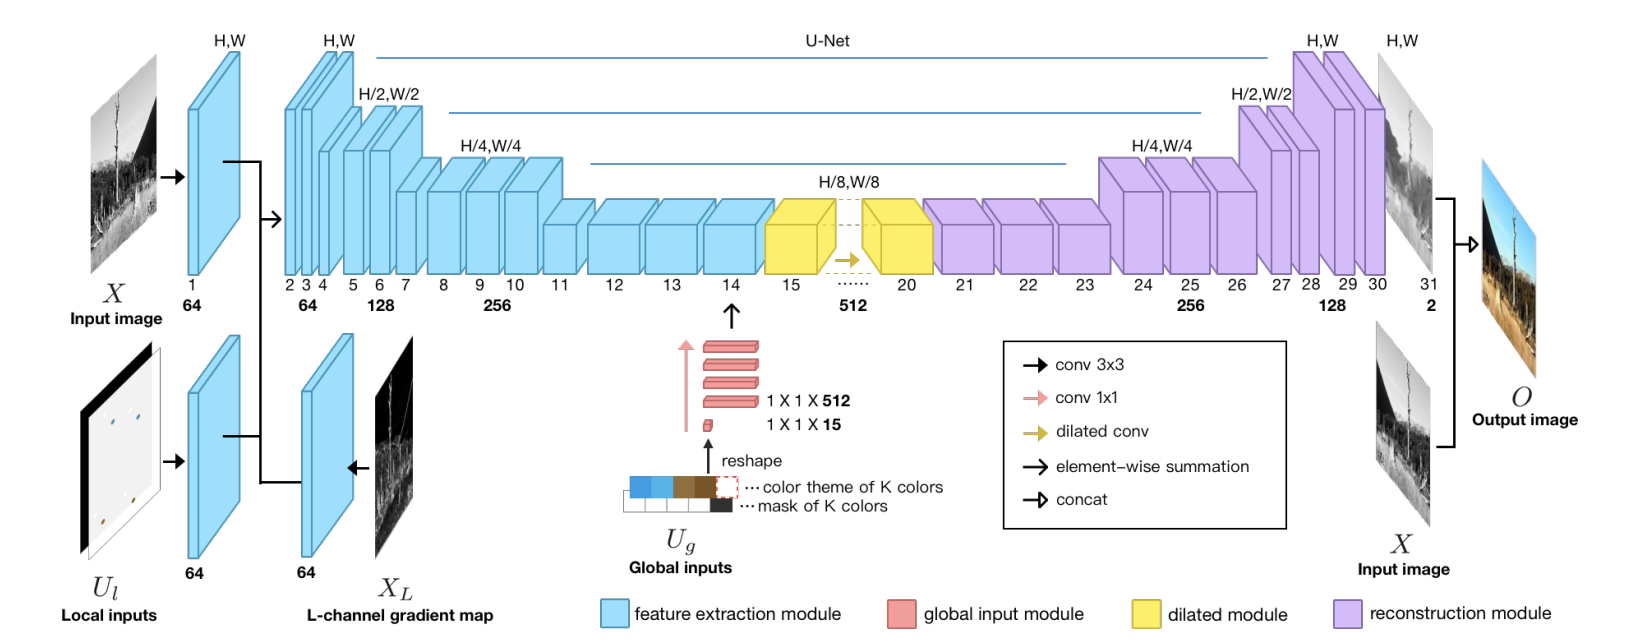
\includegraphics[totalheight = 2.5in]{zhang2017style.png}}
    \caption{整体、局部交互网络结构图}
    \label{zhang2017style}
    \end{figure*}
\subsection{基于色彩信息输入的交互上色}
线稿上色在本世纪初取得了很多不错的研究成果,其中基于数学的算法无需高算力GPU就能提供稳定的线稿上色。Yingge Qu 等在2006年提出的Manga colorization\cite{qu-2006-manga}有效地对包含大量笔画、阴影、半色调和加网的黑白漫画进行着色,由用户进行涂鸦,算法使用Gabor 小波滤波器获得基于统计的局部图案特征来测量图案连续性,然后通过监视模式连续性的水平集方法传播边界,根据这些信息对线稿精准分割并上色。Daniel Sýkora等在2009年提出的LazyBrush\cite{sykora2009lazybrush}兼容多种类型的手绘卡通作品上色,基于图论的segmentation方法把上色问题建模为一个“最优化问题”,定义一个“能量函数”来形式化地定义“线稿上色”,当能量函数的值达到最小时,就实现了最优的上色效果。

随着人工智能的兴起,许多研究者将神经网络应用到线稿上色问题。例如2017年Patsorn Sangkloy等人提出的Scribbler,\cite{sangkloy2017scribbler}利用一个基于残差连接的encoder-decoder网络结构完成涂鸦线稿上色;Lvmin Zhang等人提出了基于增强残差Unet和GAN的风格迁移算法,这是一种基于范例的上色算法,其生成器网络结构如图~\ref{sangkloy2017scribbler}所示,输入为一张黑白线稿和一张彩色参考图,彩色参考图经过一个VGG16或VGG19网络提取特征,黑白线稿经过一个encoder结构后,有三个decoder与之对应,分别用于直接解码、解码添加了彩色特征的图片和获得最终的彩色图片输出。

\begin{figure}[h]
\centerline{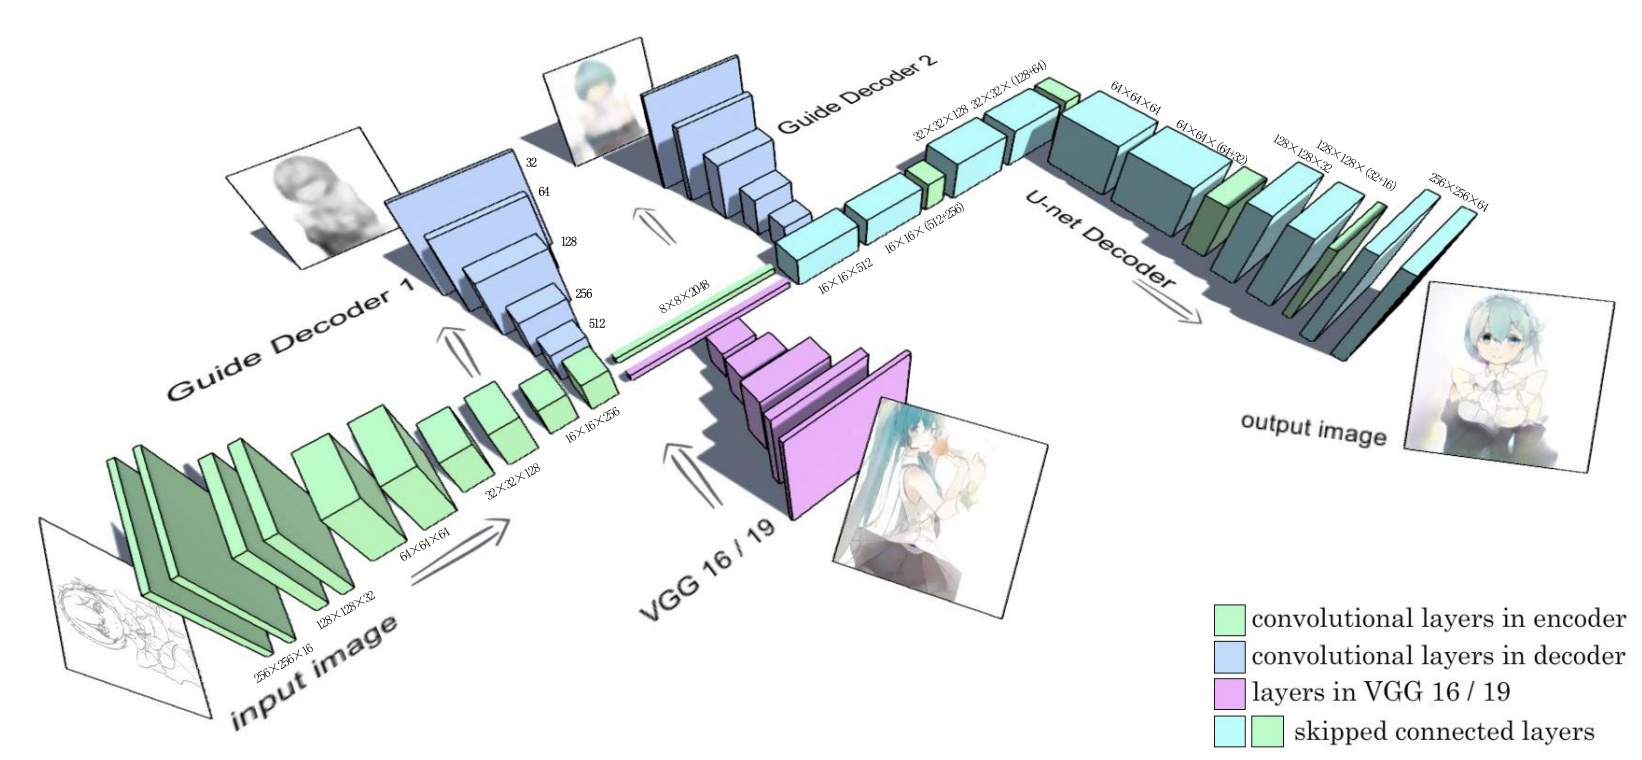
\includegraphics[totalheight = 1.6in]{sangkloy2017scribbler.png}}
\caption{Scribbler生成器网络结构图}
\label{sangkloy2017scribbler}
\end{figure}

自然图片相比于线稿包含的内容更加复杂多变,色彩连续性更强,计算复杂度也相应大幅提高,深度学习的产生为解决这类问题提供了可能。在实际操作中,对于自然图片,通常会把RGB图片转换为LAB,因为黑白的灰度图能够提供L通道的信息,仅需补充AB通道的信息。在用户干预的上色算法中,考虑到需要输入附加信息,附加信息的种类可以是局部的涂鸦也可以是整体风格,Yi Xiao等在2019年提出了一种同时支持整体参考信息输入和局部参考信息输入的深度上色网络\cite{zhang2017style},网络结构如图\ref{zhang2017style}所示,整体采用Unet结构,包括蓝色的特征提取网络,粉色的全局色彩输入网络,黄色的细节网络和紫色的特征重建网络。其中特征提取网络的输入由待处理的黑白图片、用户输入的局部信息和黑白图片L通道的梯度图三部分构成,输出为三部分结合提取到的特征,特征结合经全局色彩输入网络处理的颜色参考进入细节网络进一步处理后送入重建网络获得最终的彩色图片。这一方法的亮点在于既支持涂鸦参考信息也支持全局色彩范例,即用户既可以指定某一细节的颜色也可以指定整体颜色风格。


\subsection{基于其他信息输入的交互上色}

除了涂鸦和参考图信息作为输入,Jianbo Chen等人在2018年提出的LBIE算法\cite{chen2018language}能够实现使用文字输入指导线稿和自然图片上色;Eungyeup Kim等人在2021年提出的Deep Edge-Aware Interactive Colorization\cite{kim2021deep}先对图片进行自动上色,通过用户反馈并画出有色彩溢出的边缘从而对上色效果进行校正,有效弥补了自动上色色彩溢出的通病。
\begin{figure*}[htb]
    \centerline{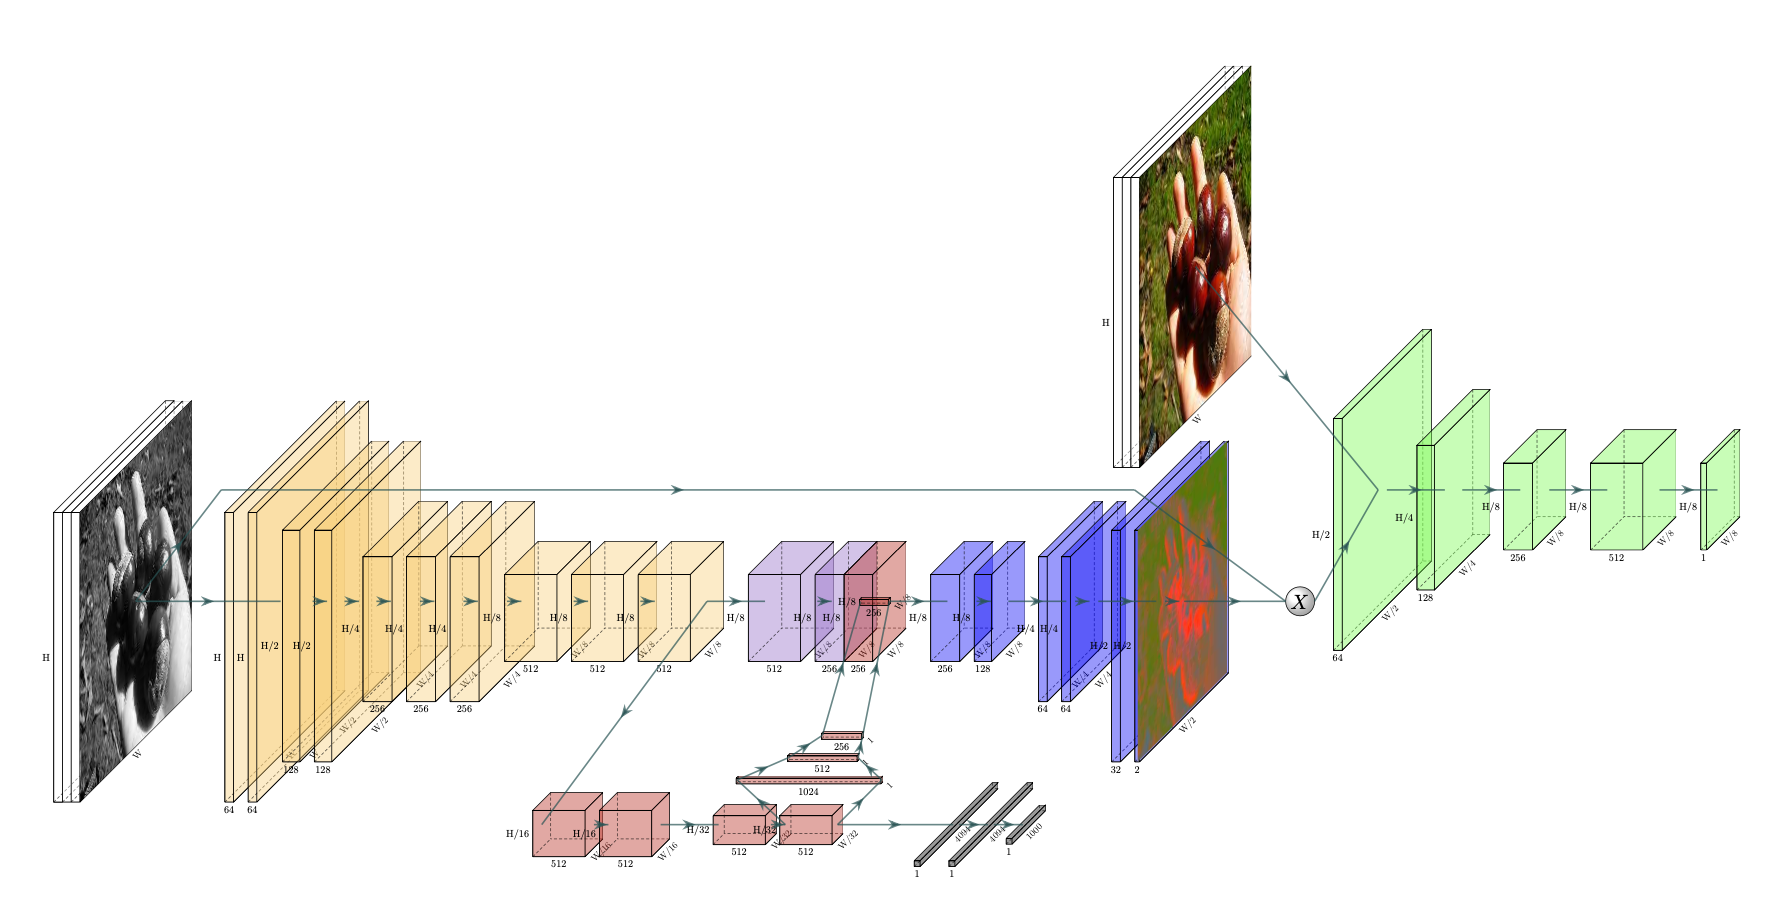
\includegraphics[totalheight = 2.5in]{2019ChromaGAN.png}}
    \caption{ChromaGAN网络结构图}
    \label{2019ChromaGAN}
    \end{figure*}
\section{完全自动上色算法}
该部分将介绍有代表性的基于深度学习的自动上色算法网络细节。

\subsection{备受欢迎的Encoder-decoder结构}
encoder-decoder结构多次出现在该领域的论文中,下面介绍三种基于encoder-decoder结构的算法。三种算法的效果在其论文发表时均达到了SOTA,且其网络结构和损失函数也有一定的相似之处。

Patricia Vitoria等人在2020年提出了ChromaGAN\cite{2019ChromaGAN},将对抗性学习方法与语义信息相结合,提出了将色彩、感知信息与语义类别分布结合在一起的三项损失函数。其网络结构如图~\ref{2019ChromaGAN}所示,左侧是生成器,分为上下两部分,上面的部分是一个encoder-decoder结构,其中黄色的encoder部分是VGG16\cite{simonyan2014very}去掉最后三个全连接层构成的,使用预训练的VGG16初始化,粉色部分是两个Conv-BatchNorm-ReLu模块;下面部分用于输出类别分布向量,红色部分由四个Conv-BatchNorm-ReLu和三个全连接层构成,灰色部分输出类分布矢量,用softmax函数生成m个语义类的概率分布特征;紫色的decoder将两个分支合并,用Conv-ReLu形式的六层网络加两次上采样处理数据得到输出图像的色度信息。右侧绿色部分是基于PatchGAN\cite{isola2017image}的鉴别器,关注局部图像块,跟踪所生成图像的高频结构。该算法的亮点在于将语义信息和对抗生存网络结合,取得了比较好的效果。

\begin{figure}[h]
    \centerline{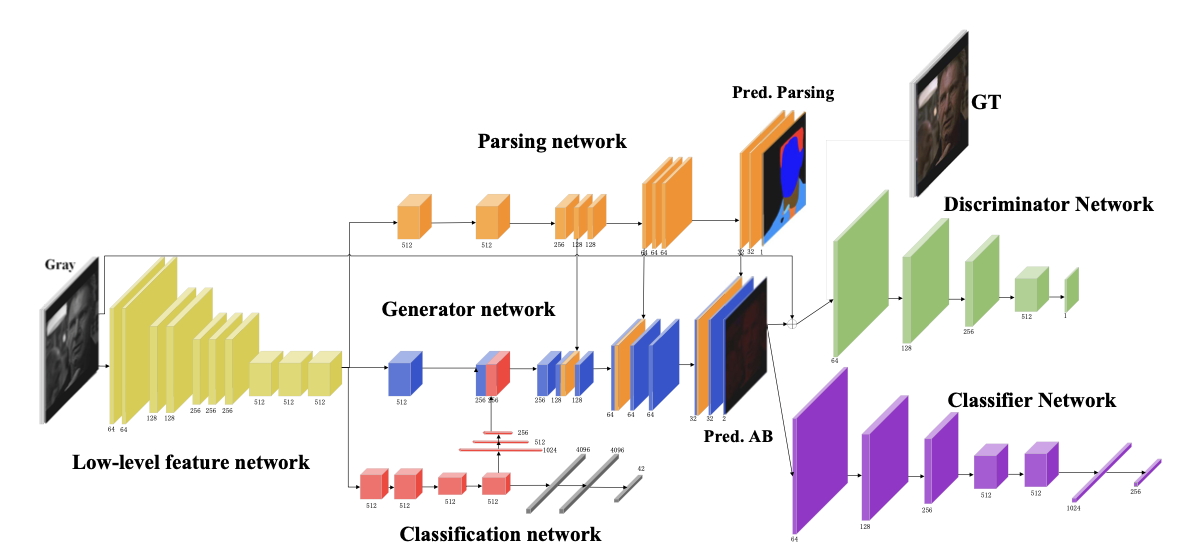
\includegraphics[totalheight = 1.6in]{jin2021focusing.png}}
    \caption{Focusing on Persons网络结构图}
    \label{jin2021focusing}
    \end{figure}

其后有Xin Jin 等人的Focusing on Persons\cite{jin2021focusing}和Yuzhi Zhao 等人的SCGAN\cite{2020SCGAN}都采用了类似的endocer-decoder结构并加入了类别分析,二者的网络结构图如图~\ref{jin2021focusing}、\ref{2020SCGAN}所示。Focusing on Persons在chromagan的基础上加入了上方的Parsing network(橙色部分)来提取人像的特征 ,同时增加了一个基于infoGAN\cite{chen2016infogan}的类别鉴别器(紫色部分)来提高网络对类别的敏感程度。

\begin{figure}[h]
    \centerline{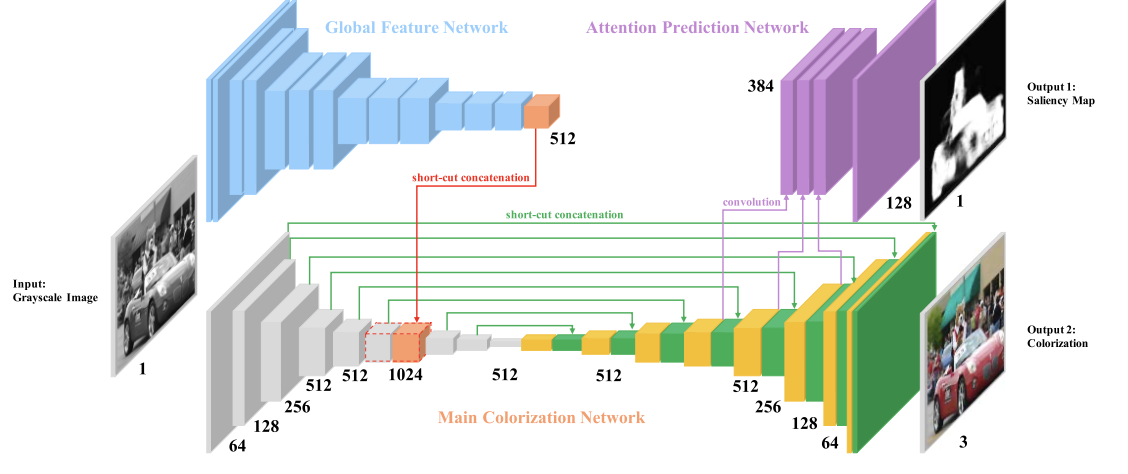
\includegraphics[totalheight = 1.5in]{2020SCGAN.png}}
    \caption{SCGAN网络结构图}
    \label{2020SCGAN}
    \end{figure}
\begin{figure*}[h]
    \centerline{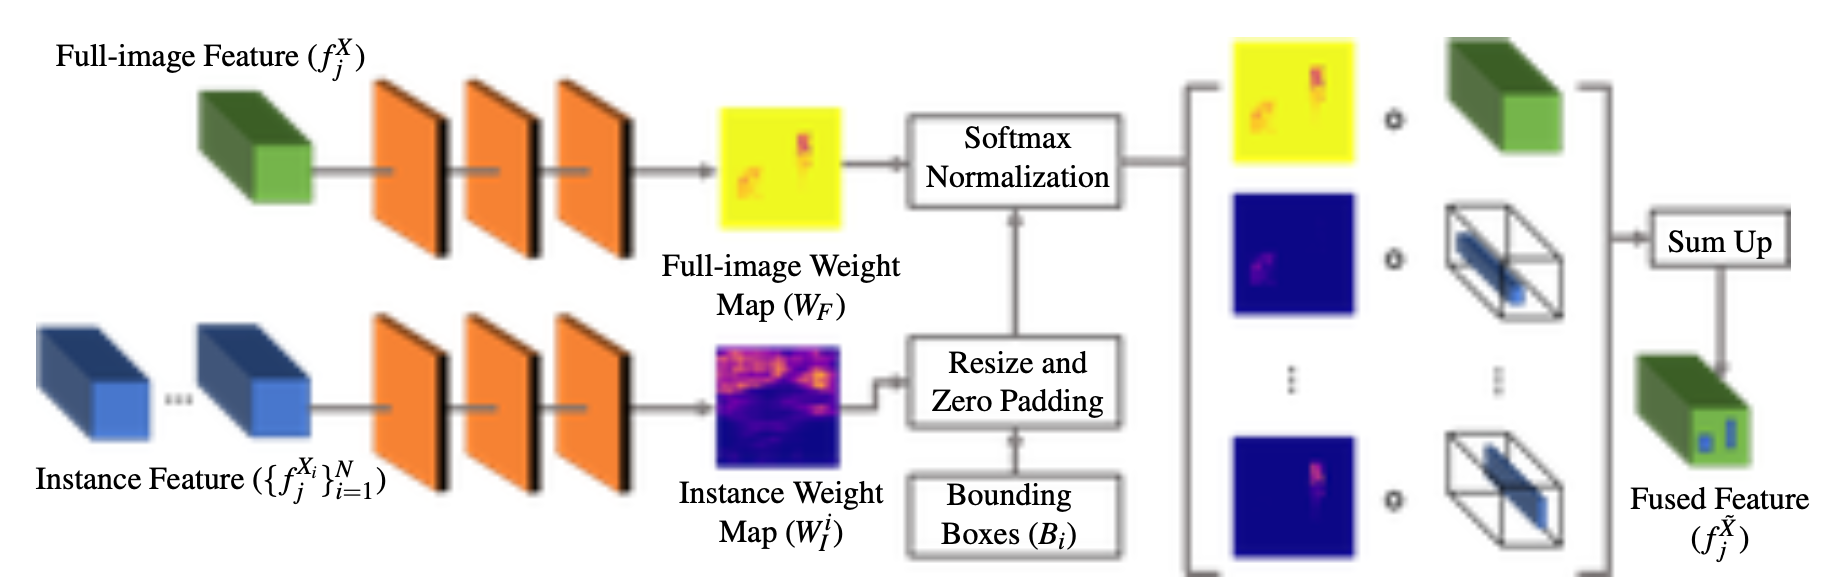
\includegraphics[totalheight = 1.6in]{2020Instance.png}}
    \caption{Instance-aware网络结构图}
    \label{2020Instance}
    \end{figure*}
SCGAN的上色主网络也是一个encoder-decoder结构,上方的Global Feature Network(蓝色部分)是一个分类网络,与ChromaGAN的encoder部分类似,都是基于VGG16\cite{simonyan2014very}分类网络调整而来,SCGAN的特殊之处在于添加了Attention Prediction Network(紫色部分)对图片的显著性区域的上色做了优化,其鉴别器使用了两个PatchGAN结构分别计算整张图片和显著性区域的loss。
\subsection{研究思路创新Instcolorization}
目前已有的网络存在一些共性问题,例如颜色偏向蓝绿色不够鲜艳、色彩溢出等,前面提到的几种算法都是用了对抗生成网络来使图片色彩尽可能鲜艳、自然,而解决这些问题除了关注上色任务本身,也有研究提出了一些解决问题的新思路,例如Jheng-Wei Su 等在2020年提出的Instance-aware Image Colorization\ref{2020Instance},网络结构如图~\ref{2020Instance}所示。

该算法为解决上色后图片整体颜色趋于一致性的问题,将目标检测、分割加入到上色网络中,将整个上色网络分为整体上色和局部上色两部分,最后训练了一个融合模型将各部分与整体上色的结果融合到一起。在目标检测分割方面,作者采用了Facebook团队开发的工具detectron2对输入的黑白图像进行目标检测、实例分割,并将分割得到的各个实例作为局部上色网络的输入;在上色方面作者使用了由Richard Zhang 等人提出的\cite{zhang2017real}当时的SOTA模型。在算法效果方面,对于比较明显的多物体图片,该模型很好的区分了不同物体的颜色风格,输出的彩色图片颜色相比其他算法更加鲜艳、有区分度,但对于不能明确划分为多个部分的图片,目标检测不能提供有效信息,此时的输出几乎仍然是黑白的。该算法上色成功与否很大程度依赖目标检测的准确程度,同时由于detectron2切割出来的目标是矩形图像块,边缘色彩溢出的问题仍然严重。虽然该方法存在很多问题,但他改变了研究思路,充分利用了开源工具和前人的优秀工作成果,对后续研究有很好的启发性。

\subsection{巧妙的问题转化}
针对自动上色缺失信息过多的问题,Yanze Wu等人\cite{wu2021towards}在2021年提出了一种非常有特点的算法,利用生成的先验色彩指导后续的上色过程,虽然也用到了encoder-decoder结构,但整体思路大不相同。

\begin{figure}[h]
    \centerline{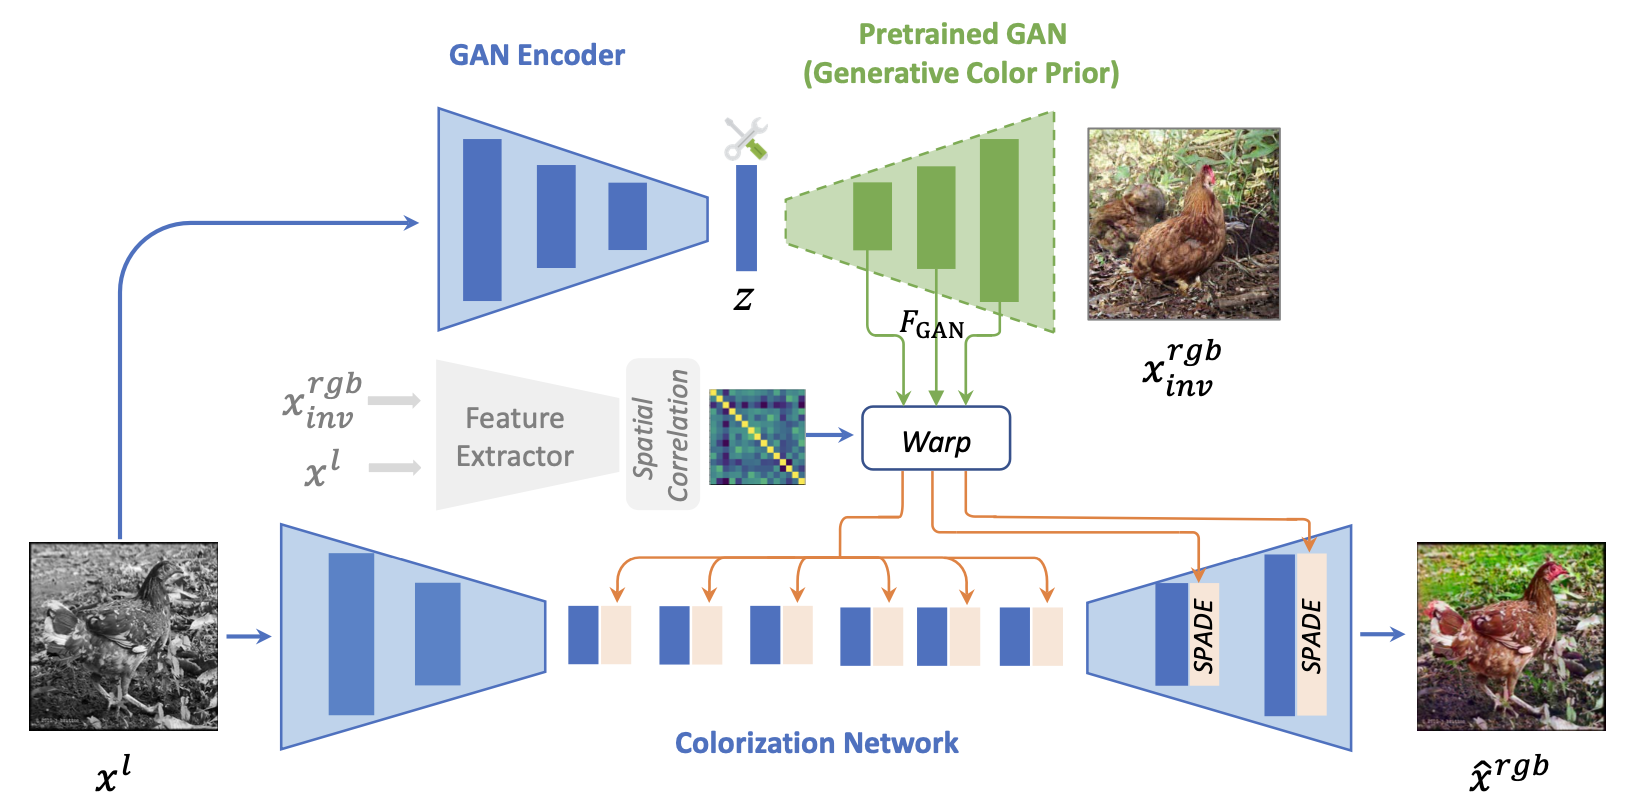
\includegraphics[totalheight = 1.6in]{wu2021towards.png}}
    \caption{先验色彩指导上色网络结构图}
    \label{wu2021towards}
    \end{figure}
其网络结构如图~\ref{wu2021towards}所示,网络包括生成色彩先验网络、上色网络、特征调制三部分。生成先验色彩网络的输入是黑白图片,经过编码器得到latent code,通过预训练的BigGAN模型得到与输入图片最相关的多尺度特征;特征调制过程将生成色彩先验网络种的多尺度特征与上色网络中黑白图片对应的多尺度特征进行空间对齐,使用SPADE方式调制上色网络;上色网络是一个普通的编解码器结构。输入黑白图片经过编码、调制、解码的过程得到最终的彩色图片输出。该算法的亮点在于跳出了使用GAN生成鲜艳色彩的思路,通过一个封装了丰富色彩信息的先验网络获取到参考图为上色提供范例,后续过程中将自动上色过程转换为基于范例的上色问题,既获得了大量参考信息,又不增加人工工作量。
\subsection{优秀的工程实践DeOldify}
最后介绍一个公认的效果较好的用于着色和恢复旧图像及视频的深度学习项目DeOldify\cite{2019deoldify},自2019年创立以来就备受关注,截至2021年12月该项目在GitHub上已有14.4k Star,上述深度学习模型的文章中多篇将模型效果与DeOldify作对比,在Instance-ware Image Colorization的论文中提到“有趣的是,虽然DeOldify并没有在基准着色实验中提供最准确的上色结果,但它的上色效果却被更多用户喜爱”\cite{2020Instance}。

DeOldify采用了一种被称作 NoGAN 的新型的、高效的图像到图像的 GAN 训练方法。细节处理效果更好,渲染也更逼真。不同于常规的GAN,NoGAN的生成器经过了常规loss的预训练而非随机生成,这使得NoGAN花费比常规GAN架构更少的训练时间。整个生成器网络架构在U-Net上使用ResNet101主干,并在其中加入了Self-attention机制以增强图片色彩的连续性。该项目已在GitHub上开源,虽然其网络结构并不复杂,但由于其训练过程中需要多次人工筛选各阶段的最优模型,对模型训练者的经验要求极高,且训练所使用的fastai框架用户较少,并未发现有基于DeOldify的相关研究,但用到的Self-attention机制可以为后续研究提供方向。

\bibliographystyle{IEEEtran}
\bibliography{papers}{}

\end{document}
